\documentclass[11pt]{article}
\usepackage[margin=1in]{geometry}
\usepackage[T1]{fontenc}
\usepackage{lmodern}
\usepackage{microtype}
\usepackage{amsmath}
\usepackage{booktabs}
\usepackage{graphicx}
\usepackage{caption}
\usepackage[section]{placeins}
\usepackage{xcolor}
\usepackage{hyperref}
\hypersetup{colorlinks=true, linkcolor=blue!50!black, urlcolor=blue!50!black}
\usepackage{enumitem}
\setlist{nosep}
\captionsetup{font=small, labelfont=bf}
\graphicspath{{../../results/report-figures/}}
\newcommand{\ttt}[1]{\texttt{\small #1}}

\title{Where DeepSeek's filler effect comes from:\\ the base checkpoint, what fills the span, and who announces it}
\author{Nick Rui \\ \small chat-model results and pipeline by Nicole; base checkpoint and all other runs from this session}
\date{September 4, 2026}

\begin{document}
\sloppy
\maketitle

\section*{The short version}

Nicole found that DeepSeek V4 Flash solves a two-step variable-binding puzzle 70\% of the time when it must answer immediately, and 98\% of the time if fifty dots sit between the question and the answer. Dots before the question do nothing. Her lens work showed intermediate values staged in the dot positions. Earlier work in this project showed that no open model up to 35B does this, and that fine-tuning one to solve the task with dots present produces a model that ignores them.

This session asked where DeepSeek's effect comes from, and got most of the way to an answer.

\begin{enumerate}
\item \textbf{The released base checkpoint does not need the dots.} Same architecture, same pretraining, no post-training: 48/50 with no filler, 50/50 with fifty dots, 49/50 with the dots before the question. There is no deficit for the dots to repair. Post-training created the 70\%.
\item \textbf{The base reads the dots the same way the chat model does.} Its answer positions put 20\% of their late attention on the dots (chat: 16\%), its dot residuals are problem-specific, and the answer is decodable from them. Reading trailing tokens is a property of the pretrained network. Needing them is what post-training added.
\item \textbf{Post-training did not remove the ability to compute at the question.} With no filler anywhere in the prompt, the chat model's last question token holds the answer exactly as well as the base's (ridge probe $R^2$ 0.84 both). The 0.40 versus 0.74 gap I first reported appears only when a filler span is present in the context.
\item \textbf{The demonstrations move the computation; the instruction sentence costs accuracy.} Five worked examples with a span between question and answer, and no span in the target, drop the chat model's question-token encoding from 0.84 to 0.40 while leaving accuracy alone. The system sentence announcing the span leaves the encoding alone and costs six items. The base reacts to neither until the shown span is fifty dots long, and then only half as much. The effect is graded by the span length the examples show.
\item \textbf{Numbers work as filler as well as dots; letters work less; order never matters.} Attention on the filler tracks the gain (letters 0.11, dots 0.16, numbers 0.23) and the ordering is the same in the base, so which token kind gets read is pretrained.
\item \textbf{Adjacent-position cosine finds no point where the model changes thought.} Every consistent drop in the series is a tokenization artifact. After removing position identity, DeepSeek's filler positions are nearly independent of their neighbors; the trained Qwen that ignores its dots carries one constant vector along the span.
\end{enumerate}

My reading: the chat model learned, in post-training, to treat the span after a question as the place where arithmetic gets finished, and to calibrate how much it defers to how long a span the context leads it to expect. Given a span, it finishes there and scores 98\%. Given none, it emits an approximate answer with low confidence and scores 70\%. The base has the same reading machinery and no such habit, so it finishes at the question and scores 96\% either way.

\tableofcontents

\section{What was already known}

\subsection{The task and Nicole's result}

Each item defines five variables, some as numbers and some as ``twice the number for X plus 3'', then asks for a two-step expression over one of them. The model sees five worked demonstrations and must answer with a number and nothing else. The filler condition inserts $k$ dots between the question and the ``Answer:'' cue, with a sentence in the system prompt saying exactly how many filler tokens will appear. Nicole ran the released 50 items on DeepSeek V4 Flash: 35/50 at $k=0$, 49/50 at $k=50$, 35/50 with the fifty dots placed before the question instead. Her logit-lens and patching work showed the values of the two arithmetic steps appearing in the dot positions at increasing depth and being read out late.

\subsection{The earlier null on open models}

Before this session I had run the same items through ten open models from 4B to 35B and through several LoRA fine-tunes of Qwen3.5-9B trained with dots present. None showed a placement-specific filler gain. The fine-tuned models solved the task at the answer position and treated the dot positions as inert: their dot residuals decoded to the dot token, could be wiped at every block without changing the answer, and received 1 to 4\% of the answer position's attention. On DeepSeek's chat model the same anatomy showed the opposite: 16 to 43\% of late attention on the dots, problem-specific dot residuals, and the answer decodable from the dots (0.87) but barely from the question token (0.40). That left one question: is this the architecture (DeepSeek's four-stream residual and sliding-window attention) or the post-training? The base checkpoint answers it.

\subsection{Setup for everything below}

All DeepSeek runs use Nicole's 4-way model-parallel loader on a 4$\times$H100 80\,GB box. Behavior is measured on the released 50 items; anatomy on 50 held-out items at $k=50$ (filler counted in items; a number is two tokens on DeepSeek's tokenizer). Probes are ridge regressions in dual form with 5-fold item-level cross-validation, reporting $R^2$ for the answer from a position's residual; the best block is reported. Attention is recomputed from $q$, $k$, the indexer's selection and the per-head sink, because the fused sparse-attention kernel returns no weights; keys are attributed to prompt regions (prefix, problem, filler, template, and later the announcement sentence and the demonstrations' spans). ``Chat rendering'' is DeepSeek's turn-marker template; ``plain rendering'' is raw few-shot text. Statistics are exact McNemar tests on paired items.

\section{The base checkpoint}

\subsection{Getting it to run}

\ttt{DeepSeek-V4-Flash-Base} ships FP8 experts where the chat checkpoint ships FP4, so the converted shards are 75\,GB per GPU against 42\,GB. They fit on 79\,GiB cards only with \ttt{PYTORCH\_ALLOC\_CONF=expandable\_segments:True}: the default caching allocator rounds every 8\,MiB expert weight into a 20\,MiB segment and loses about 12\,GiB per GPU, which is the whole margin. Loaded through the chat repository's reference code with the expert dtype unset, the sanity gate (final-head closure, lens identity anchor) passed with no failed prompts. Prompts are token-for-token identical to Nicole's run (checked: 300 of 300).

\subsection{Behavior}

\begin{table}[h]\centering\small
\begin{tabular}{lrrrrrr}\toprule
Correct of 50 & $k$=0 & 5 & 10 & 25 & 50 & 100 \\ \midrule
chat (Nicole) & 35 & 45 & 42 & 43 & 49 & 49 \\
base, chat rendering & 48 & 48 & 49 & 49 & 50 & 49 \\
base, plain rendering & 47 & 44 & 50 & 47 & 50 & 50 \\ \bottomrule
\end{tabular}
\caption{Released items, post-question dots. Pre-question fifty dots: chat 35, base 49 (chat rendering) and 50 (plain).}\end{table}

The base is at ceiling with or without dots, in either placement, in either rendering. Helped-minus-hurt is at most two items anywhere. The chat model's 70\% is a deficit that post-training introduced, and fifty dots bring it back to the base's level.

\subsection{Anatomy}

\begin{figure}[h]\centering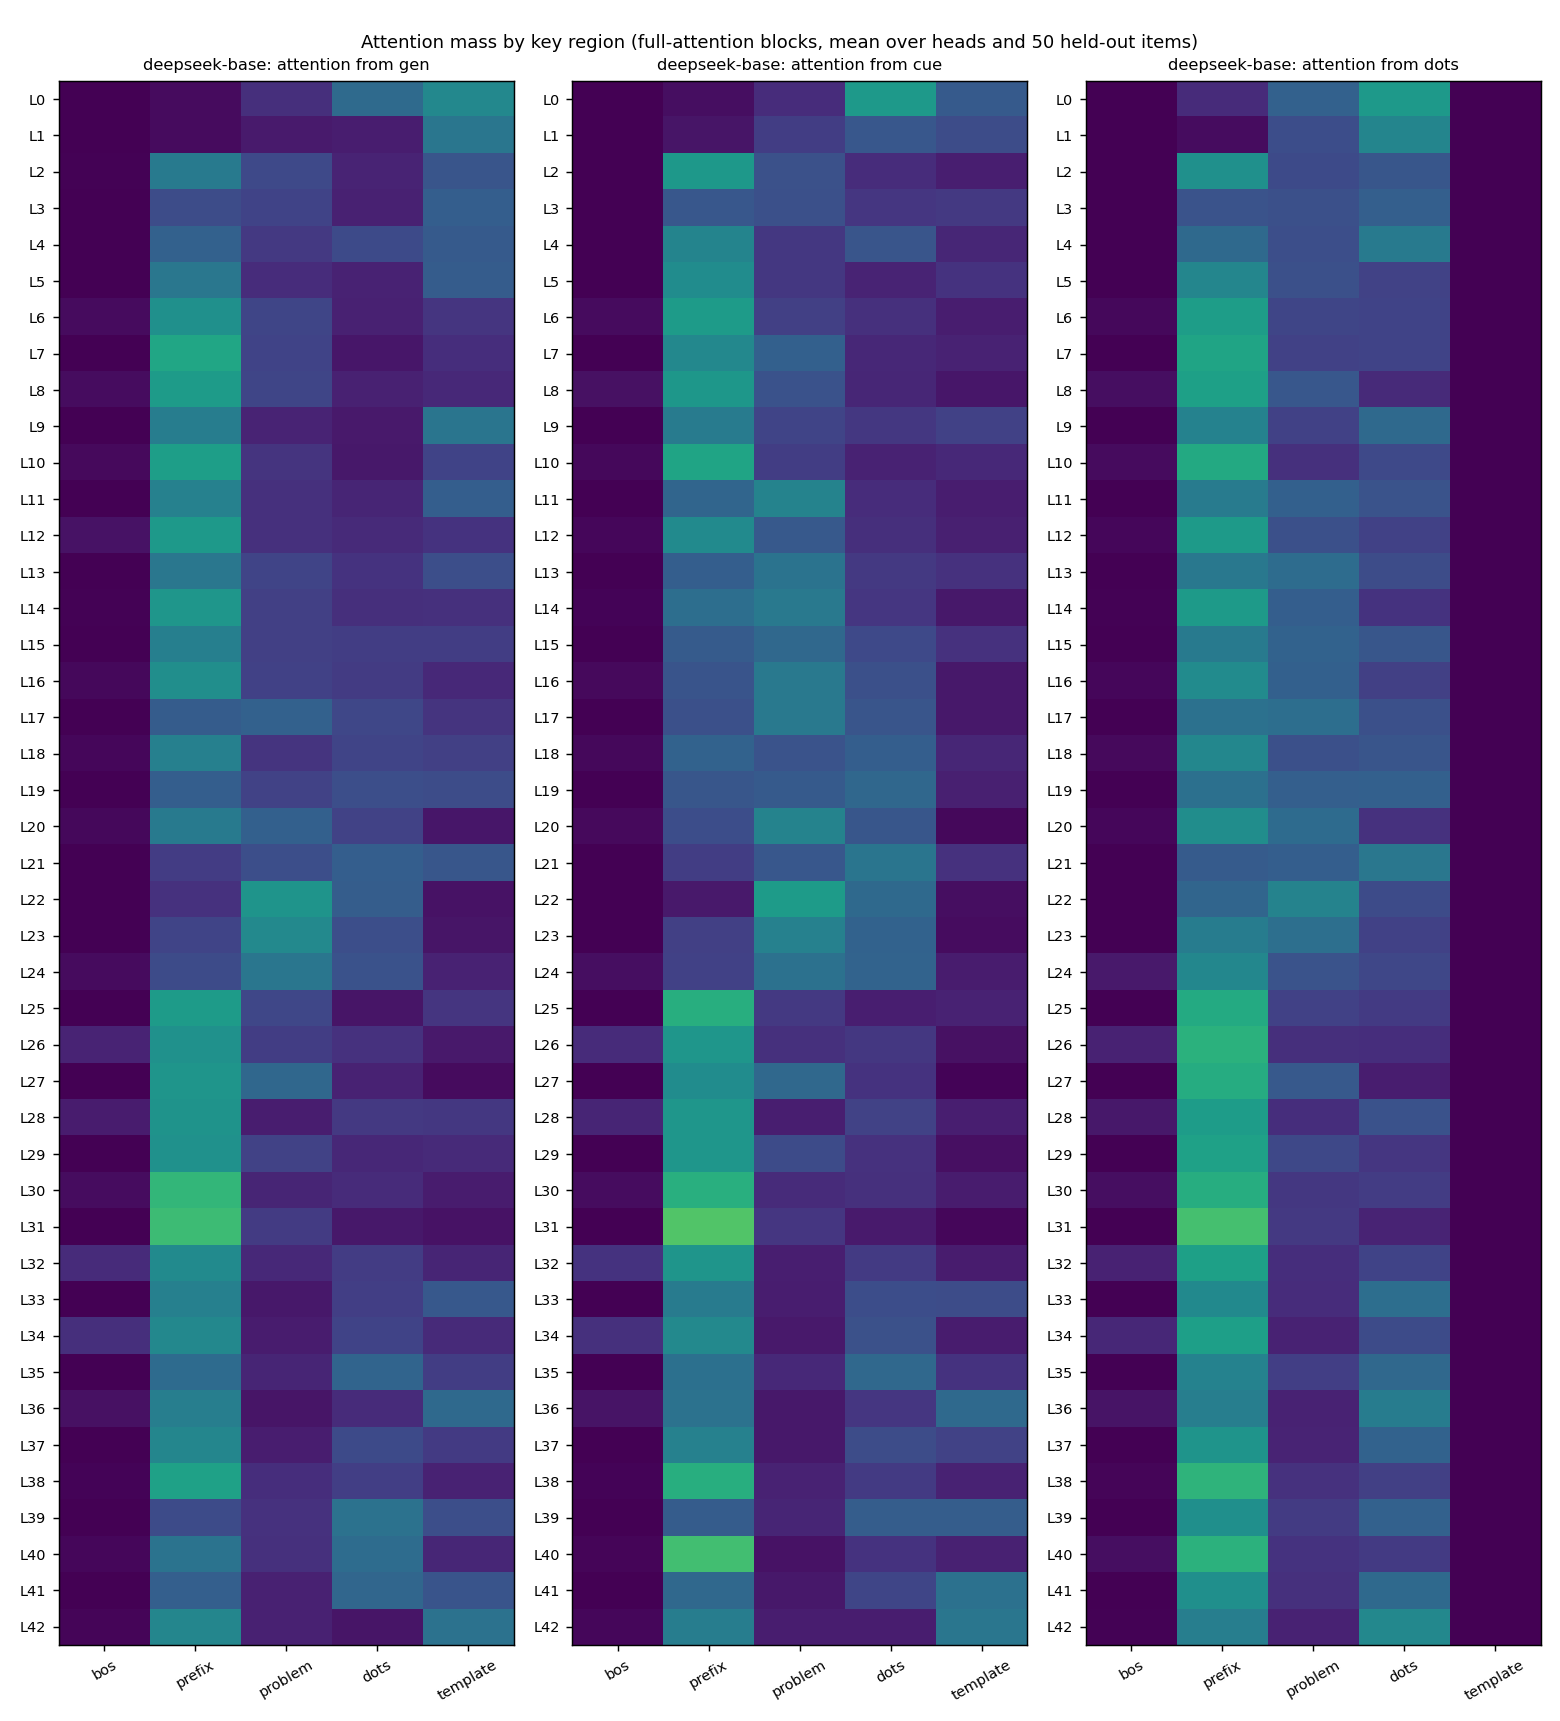
\includegraphics[width=0.85\textwidth]{deepseek_base_attention_heatmaps.png}
\caption{Base checkpoint: attention mass by key region at every block, from the generation position, the answer cue, and the dots. The chat model's figure looks the same.}\end{figure}

\begin{table}[h]\centering\footnotesize
\begin{tabular}{lrrrrr}\toprule
 & gen $\to$ dots & cue $\to$ dots & cos same dot, other items & $R^2$ ans$|$dots & $R^2$ ans$|$question token \\ \midrule
chat & 0.164 & 0.195 & 0.78 & 0.87 & 0.40 \\
base & 0.203 & 0.189 & 0.64 & 0.85 & 0.74 \\ \bottomrule
\end{tabular}
\caption{Fifty held-out items at $k=50$. Attention is the mean mass on the dot region over the last third of blocks.}\end{table}

The base reads the dots at least as hard as the chat model, in the same blocks, with more heads above half their mass on dots. Its dot residuals are more problem-specific. The four hyper-connection streams divide the work the same way (two content lanes, one position lane, one carrier). Everything in the chat model's anatomy that looked like a workspace is already there before post-training. The one column that separates the checkpoints is the answer at the question token: 0.74 in the base, 0.40 in chat.

\subsection{What the chat model gets wrong}

All fifteen of its $k=0$ misses are numbers of the right magnitude. None is a wrong-variable substitution: I resolved every variable in each prompt and applied the final operation to each, and no miss matches. Nine of fifteen are within 4 of the answer, one drops the doubling, one drops the constant. The first-token distribution is three times flatter than the base's (top-10 entropy 0.76 versus 0.30 nats), the correct number sits at median rank 3 on a miss, and fifty dots sharpen the distribution to the base's level (0.26). The model always finds the right chain and emits an imprecise result with low confidence. ``Forgot'' is the wrong word; ``relocated'' turned out to be the right one, for the reason in Section 5.

\section{What fills the span}

\ttt{src/jlens\_filler/prompts.py} renders dots, the alphabet, a fixed scrambled alphabet, counting numbers, and a fixed scrambled sequence of numbers. Same 50 items, same scaffold, chat rendering.

\begin{table}[h]\centering\scriptsize
\begin{tabular}{llrrrrrrll}\toprule
Filler & Model & $k$=0 & 5 & 10 & 25 & 50 & 100 & helped/hurt @50 & pre-question @50 \\ \midrule
dots & chat & 35 & 45 & 42 & 43 & 49 & 49 & 14/0 & 35 \\
alphabet & chat & 34 & 41 & 43 & 41 & 42 & 43 & 12/4 & 34 \\
alphabet, scrambled & chat & 34 & 38 & 32 & 38 & 41 & 46 & 10/3 & 36 \\
counting & chat & 34 & 45 & 45 & 46 & 49 & 48 & 15/0 & 35 \\
counting, scrambled & chat & 34 & 31 & 41 & 41 & 49 & 50 & 15/0 & 28 \\
any type & base & 48 & 48--50 & 49--50 & 48--50 & 49--50 & 49--50 & $\leq$2/1 & 49--50 \\ \bottomrule
\end{tabular}
\caption{Correct of 50 by filler type. Numbers are two tokens each on this tokenizer, so 50 numbers are 99 tokens.}\end{table}

Numbers work as well as dots, scrambled or not. Letters help less, scrambled or not, and 100 letters (100 tokens) still trail 50 numbers (99 tokens), so this is not token count. Scrambled numbers hurt at $k=5$ before helping. Every type is placement-specific. The base is at ceiling for every type.

\begin{table}[h]\centering\scriptsize
\begin{tabular}{llrrrrr}\toprule
Model & Filler & gen$\to$filler & cos same pos & $R^2$ ans$|$filler & $R^2$ ans$|$question token & correct @50 \\ \midrule
chat & dots & 0.164 & 0.78 & 0.87 & 0.40 & 49 \\
chat & alphabet & 0.126 & 0.82 & 0.84 & 0.24 & 42 \\
chat & alphabet, scrambled & 0.113 & 0.85 & 0.83 & 0.43 & 41 \\
chat & counting & 0.227 & 0.77 & 0.89 & 0.51 & 49 \\
chat & counting, scrambled & 0.231 & 0.77 & 0.91 & 0.52 & 49 \\
base & dots & 0.203 & 0.64 & 0.85 & 0.74 & 50 \\
base & alphabet & 0.180 & 0.77 & 0.83 & 0.88 & 50 \\
base & alphabet, scrambled & 0.164 & 0.81 & 0.78 & 0.87 & 50 \\
base & counting & 0.271 & 0.72 & 0.82 & 0.78 & 49 \\
base & counting, scrambled & 0.267 & 0.72 & 0.88 & 0.76 & 50 \\ \bottomrule
\end{tabular}
\caption{Anatomy by filler type, 50 held-out items, $k=50$ items.}\end{table}

Attention on the filler tracks the chat model's gain: letters 0.11 to 0.13 and 41 to 42 correct, dots 0.16 and 49, numbers 0.23 and 49. The base reads every type harder than the chat model, in the same order, so which token kind attracts the answer positions is pretrained; post-training scaled it down without changing the ranking. The answer is decodable from every filler type in both checkpoints, and the checkpoints again separate only at the question token, for all five fillers.

A note on decodability. Llama-3.1-8B-Instruct and Gemma-3-27B-IT, which get nothing from dots and put 1 to 2\% of attention on them, also hold the answer in their dot residuals at 0.84 and 0.81. A residual stream leaks its context; decodability of the answer from the span is not evidence the span is used. Attention from the answer positions and the non-redundancy of the span (next section) are what separate DeepSeek from every non-using model.

The same fillers on Qwen3.5-9B: the untrained model is at floor for all of them. The LoRA trained only on dot prompts gets nothing from letters and is hurt by numbers (42 $\to$ 37; scrambled 42 $\to$ 30, twelve items hurt and none helped). Its answer position ignores dots and letters (attention 0.01) but attends to filler digits at 0.05 with single heads at 0.5: a model that does its arithmetic at the answer position reads filler digits as problem digits.

\section{Adjacent-position cosine: is there a point where the model changes thought?}

For each item, the residual at every filler position and every block. Adjacent cosine is $\cos(h_p, h_{p+1})$ per block and flattened over blocks. The \emph{item-centered} version subtracts the per-position mean over items first, which removes the position-identity component that dominates filler residuals (97\% of variance in the trained Qwen) and leaves the problem-specific content. Change points are boundaries where an item's flattened centered series drops more than two standard deviations below its own mean.

\begin{figure}[h]\centering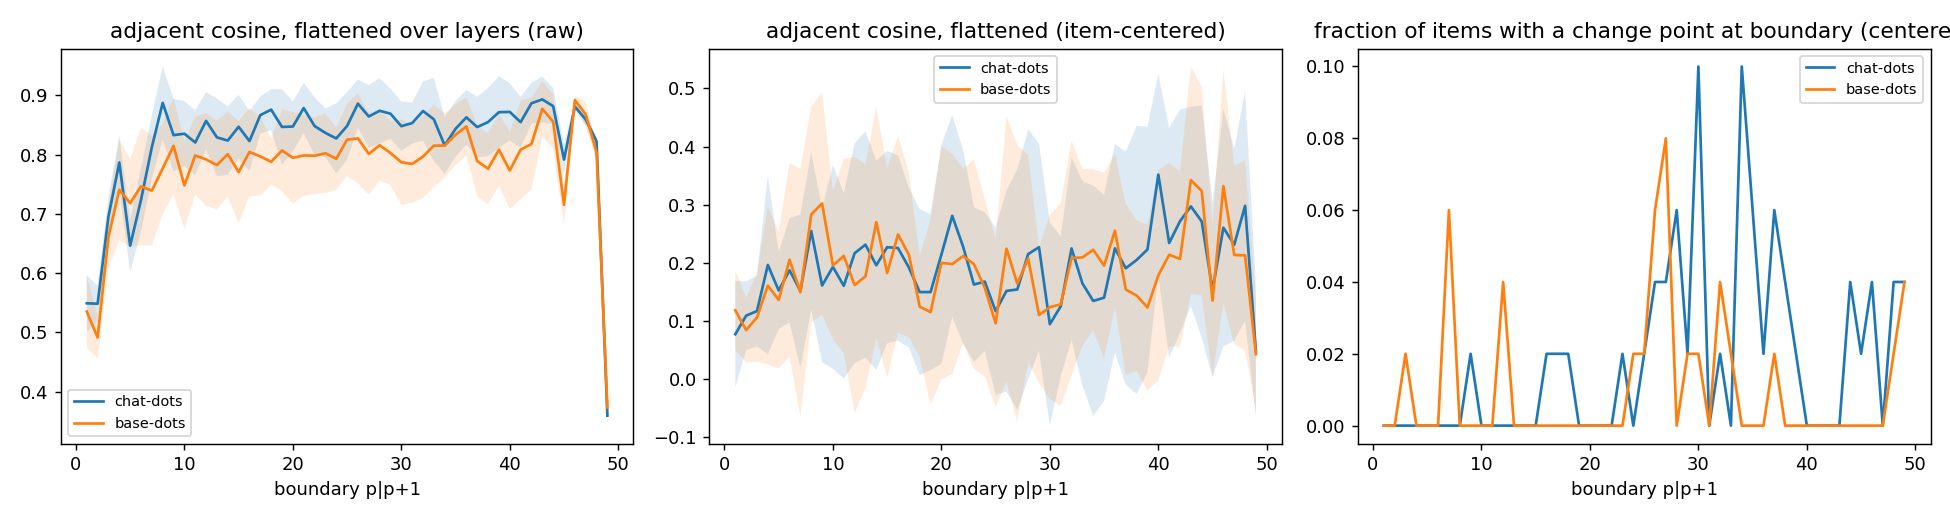
\includegraphics[width=\textwidth]{deepseek_adjacent_cosine_flat.png}
\caption{Fifty dots, chat versus base: adjacent cosine flattened over blocks (left), item-centered (middle), fraction of items with a change point at each boundary (right).}\end{figure}

\begin{table}[h]\centering\footnotesize
\begin{tabular}{lp{2.6cm}rp{4.4cm}}\toprule
Model (dots) & centered adjacent cosine, late blocks & change pts/item & where \\ \midrule
Qwen3.5-9B base & 0.25 to 0.30 & 0.15 & diffuse \\
Qwen3.5-9B $k=0$-only LoRA & 0.44 to 0.51 & 0.69 & F1/2 (42 of 100 items) \\
Qwen3.5-9B dots-only LoRA & 0.75 to 0.82 & 4.2 & F2/3, F3/4 (100/100), F7/8 (98) \\
Llama-3.1-8B-Instruct & 0.44 to 0.59 & 0.44 & F4/5 (22 of 50) \\
Gemma-3-27B-IT & 0.23 to 0.36 & 0.26 & diffuse \\
DeepSeek chat & 0.06 to 0.19 & 0.88 & diffuse, none above 5 of 50 \\
DeepSeek base & 0.06 to 0.19 & 0.48 & diffuse, none above 4 of 50 \\ \bottomrule
\end{tabular}
\caption{How much problem-specific content one dot shares with the next.}\end{table}

Three findings. First, every consistent drop in the raw series is tokenization: the first dot has no leading space, the last merges with the newline, the alphabet wraps from z to a at F26$|$F27, and number fillers alternate number, space. Between artifacts the raw adjacent cosine is 0.7 to 0.96 and flat. Second, after centering, DeepSeek's filler positions share 0.01 to 0.19 of their problem content with their neighbors, for every filler type, and change points are scattered with no boundary shared by more than five items. The span is fifty weakly related snapshots, not a trajectory with segments. Third, the trained Qwen that ignores its dots carries one constant problem vector along the span (0.77) with a settling transient in the first ten dots identical across all 100 items. That signature needs identical tokens (it falls to 0.08 to 0.23 with letters or numbers), so redundancy is compared within a filler type; within dots the contrast stands.

I do not think ``change of thought'' is the right frame for what happens in the span. Nothing pivots. The content at each position is mostly its own.

\section{Who announces the span}

\subsection{No filler anywhere}

The 0.74 versus 0.40 probe gap of Section 2 was measured with fifty dots present. Dumping both checkpoints at $k=0$, with no filler sentence, no filler in the demonstrations and none in the target, gives 0.84 at the question token for both. The question token precedes the dots, so the dots cannot cause the gap. What differs between the $k=0$ and $k=50$ prompts is the system sentence announcing fifty filler tokens and the five demonstrations that contain them.

\subsection{Announced but absent}

\ttt{extract\_dsv4.py -{}-announce-filler N} renders the sentence and the demonstrations with $N$ dots and the target with none.

\begin{table}[h]\centering\small
\begin{tabular}{lrrrrr}\toprule
Announced dots, none delivered & 0 & 5 & 25 & 50 & 50, delivered \\ \midrule
chat: $R^2$ answer at question token & 0.84 & 0.51 & 0.36 & 0.31 & 0.36 \\
base: $R^2$ answer at question token & 0.84 & 0.86 & 0.85 & 0.55 & 0.65 \\
chat: correct of 50 & 34 & & & 32 & 49 \\
base: correct of 50 & 48 & & & 46 & 50 \\ \bottomrule
\end{tabular}
\caption{Deferral is triggered by the context and graded by the announced count. Probes at the cue and generation positions stay at 0.79 to 0.83 in every condition.}\end{table}

The chat model defers in proportion to the span it is led to expect: five promised dots halve its in-place computation, twenty-five bring it to the fifty-dot level. The value is assembled at the cue and generation positions instead. The base ignores the announcement until fifty and then defers partly. Accuracy moves far less than the probe (34 to 32), so deferral is not itself the $k=0$ deficit, and no linear probe at any position sees that deficit: the answer is decodable at the generation position at 0.84 in both checkpoints in every condition, yet one emits it right 96\% of the time and the other 68\%. That is a precision-of-emission problem sitting on top of an approximately correct linear representation, which matches the near-miss pattern.

\subsection{Which channel}

\ttt{announce\_mode} splits the announcement into its two channels.

\begin{table}[h]\centering\small
\begin{tabular}{lrrrr}\toprule
Target $k=0$, announced by & chat: probe & chat: correct & base: probe & base: correct \\ \midrule
nothing & 0.84 & 34 & 0.84 & 48 \\
sentence only & 0.83 & 28 & 0.84 & 50 \\
demonstrations only & 0.40 & 34 & 0.55 & 46 \\
both & 0.31 & 32 & 0.55 & 46 \\ \bottomrule
\end{tabular}
\caption{A double dissociation.}\end{table}

The demonstrations move the computation off the question token and leave accuracy alone. The sentence leaves the question token alone and costs the chat model six items, its worst score in any condition, while the base is unaffected. The grading is the demonstrations' too: with demonstrations alone showing 5, 25, 50 dots, the chat probe is 0.49, 0.33, 0.40 and the base's 0.84, 0.82, 0.55.

So the deferral is in-context format learning. Five examples of question, span, answer teach both checkpoints, the chat model far more strongly, to finish the arithmetic after the question rather than at it, in proportion to the span the examples show. The instruction sentence is a different thing: it degrades the post-trained model's answer without changing where the answer is computed, and it does nothing to the base.

With fifty dots actually delivered, the same split governs how useful they are: nothing announced 34 $\to$ 39, sentence only 28 $\to$ 36, demonstrations only 34 $\to$ 47, both 34 $\to$ 49. Unannounced dots help a little. Examples of a span being used make them work. The sentence adds the last two items on top.

\subsection{Where the two channels are read}

Attributing attention keys to the 21-token filler sentence: from the question token, the chat model puts 0.04 of its attention on it in blocks 20 to 24 (single heads at 0.16), 0.06 in blocks 26 to 38 (a head at 0.25), and 0.17 at block 40 (a head at 0.38), against a uniform-attention level of 0.026. The base stays at or below 0.009 through block 36 and reads it at 0.08 at block 40. The sentence is about 600 tokens before the question, outside the 128-token window, so this is attention through the compressed keys. Post-training installed heads that read the instruction; given the channel result, they are the route to the sentence's cost to accuracy, not the deferral mechanism.

The demonstrations' spans, by contrast, are not read specially. Under demonstrations-only announcement the question token's attention on the demonstrations' 250 filler tokens is 0.16 (chat) and 0.21 (base), at or below those tokens' share of the keys (about 0.32), and the two checkpoints do not differ. Whatever the demonstrations do to the question token's computation, it is not carried by attention from the question token to the spans. That mechanism is still open.

\subsection{Two more checks}

Plain rendering (no turn markers, no think tag) drops the chat model to 19/50 at $k=0$ and dots still lift it to 44 at $k=100$. The chat template was helping, so ``the format interferes'' is out, and the dot effect survives a change of rendering. And the confidence picture holds: announcing absent filler flattens the chat model's first-token distribution further (entropy 1.13 nats), dots sharpen it (0.26).

\section{What this adds up to}

\paragraph{On DeepSeek.} The filler effect is post-training's. The base has the dot-reading anatomy and no deficit. The chat model has the same anatomy plus a habit: shown examples with a span, it moves its arithmetic into the span it expects, in proportion to the span's length, and emits an imprecise low-confidence answer if the span never comes. The instruction sentence is a separate small tax on the post-trained model. This is consistent with reasoning-oriented reinforcement learning that rewards working in the tokens after the question, and it explains the placement specificity: dots before the question are not a span after it.

\paragraph{On what fills the span.} Any token kind the answer positions will read works. Numbers are read hardest and work best; letters least and worst; order is irrelevant. The ranking is pretrained.

\paragraph{On method.} Three results are cautions for anyone doing this kind of analysis. Linear decodability of the answer from filler is not evidence the filler is used (Llama and Gemma). A rising filler-to-answer cosine along the span is not either (the dots-only Qwen has it). And an attention footprint on an instruction is not the mechanism of the behavior the instruction correlates with (the sentence-reading heads).

\section{Limitations}

\begin{itemize}
\item Fifty items per condition. Behavioral differences of two or three items are noise; the ones I lean on are ten or more with exact McNemar $p<0.01$, or probe differences of 0.3 or more.
\item Ridge probes at $R^2$ 0.84 have residual errors of tens of units on three-digit answers and cannot separate exact from off-by-a-few. The $k=0$ emission deficit is beyond what linear probes can show.
\item Attention is recomputed outside the fused kernel and attributed to regions; compressed keys are spread evenly over the tokens they pool. Region masses are approximate at the block level and exact at the window level.
\item The two channels were separated at the prompt level. Nothing here is a causal intervention on the network: the sentence-reading heads were located, not ablated; the demonstrations' mechanism was not found.
\item The exact-count sentence says ``50 filler tokens'' for number fillers that are 99 tokens; noted, not fixed.
\end{itemize}

\section{What I would do next}

\begin{enumerate}
\item Ablate the sentence-reading heads' attention to the announcement (blocks 20 to 40, question token) and see whether the chat model's sentence-only accuracy (28) returns to 34.
\item Find the demonstrations' mechanism. Candidates: patch the question-token residual from a demonstrations-only run into an unannounced run at each block and watch the probe; or vary the demonstrations one at a time (span in one example, in three, in five) to see whether deferral accumulates.
\item Characterize the emission deficit directly: teacher-force the correct answer and compare the chat and base models' logit margins at the first digit, with and without a span.
\item If DeepSeek publishes intermediate post-training checkpoints, run the demonstrations-only probe on each; the point where 0.84 becomes 0.40 is where the habit was learned.
\end{enumerate}

\appendix
\section{Artifacts}
\begin{raggedright}
\begin{itemize}
\item Running log with every table: \ttt{reports/\allowbreak filler-types-and-cosine.md}; base checkpoint write-up: \ttt{reports/\allowbreak small-open-model-null-result.md} and Parts V to VII of \ttt{reports/\allowbreak pdf/\allowbreak filler-tokens-open-models.pdf}.
\item Chains: \ttt{scripts/\allowbreak run\_dsv4\_base\_eval.sh}, \ttt{run\_dsv4\_base\_dot\_dump.sh}, \ttt{run\_dsv4\_filler\_types.sh}, \ttt{run\_hf\_filler\_types.sh}, \ttt{run\_dsv4\_followups.sh}, \ttt{run\_dsv4\_announce.sh}, \ttt{run\_dsv4\_announce\_graded.sh}, \ttt{run\_dsv4\_announce\_channels.sh}, \ttt{run\_dsv4\_channels\_delivered.sh}, \ttt{run\_dsv4\_demos\_graded.sh}, \ttt{run\_dsv4\_announce\_attention.sh}, \ttt{run\_dsv4\_demo\_attention.sh}, \ttt{run\_hf\_other\_models\_cosine.sh}.
\item Analysis: \ttt{analyze\_dot\_residuals.py}, \ttt{analyze\_filler\_cosine.py}, \ttt{summarize\_filler\_types.py}, \ttt{probe\_k0\_dump.py}, \ttt{summarize\_announce\_attention.py}.
\item Harness changes: filler types and \ttt{target\_length} / \ttt{announce\_mode} in \ttt{src/\allowbreak jlens\_filler/\allowbreak prompts.py}; \ttt{-{}-render plain}, \ttt{-{}-announce-filler}, \ttt{-{}-announce-mode} in \ttt{extract\_dsv4.py}; $k=0$ and announcement support plus new key regions in the two DeepSeek dump scripts.
\item Results directories: \ttt{results/\allowbreak deepseek-v4-flash\{,-base\}/} (per condition), \ttt{results/\allowbreak filler-cosine/} (cross-condition tables), \ttt{results/\allowbreak qwen3.5-9b/\allowbreak filler-types/}, \ttt{results/\allowbreak llama3.1-8b-it/}, \ttt{results/\allowbreak gemma-3-27b-it/}.
\item Raw residual and attention dumps for every condition (60 files, 86\,GB): private Hugging Face dataset \ttt{nick-rui/\allowbreak jlens-filler-dumps}, same layout as \ttt{results/}.
\end{itemize}
\end{raggedright}

\end{document}
